\section{Exemples avec les packages \tkzname{alterqcm} et \tkzname{tkz-tab}}


\shorthandoff{:}
\begin{alterqcm}[lq=110mm]

\AQmessage{ La figure 1. donne la représentation graphique d'une fonction $f$ définie sur $\mathbf{R}^+$ et la figure 2 celle d'une primitive de $f$ sur $\mathbf{R}^+$.

\begin{center}
 \begin{tikzpicture}[xscale=2.25,yscale=1]
   \tkzInit[xmin=-2,xmax=3,ymin=-1,ymax=6]
   \tkzDrawX
   \tkzDrawY
   \tkzFct[samples=100,domain = -1:2.2]{x+exp(x-1)}
    \tkzDefPoint(1,2){pt1}
    \tkzDrawPoint(pt1) 
    \tkzPointShowCoord[xlabel=$1$,ylabel=$2$](pt1)
    \tkzDefPoint(2,4.71828){pt2}
    \tkzDrawPoint(pt2)  
    \tkzPointShowCoord[xlabel=$2$,ylabel=$\text{e}+2$](pt2) 
   \tkzRep   
 \end{tikzpicture}
\end{center} 

\begin{center}
  \begin{tikzpicture}[xscale=2.25,yscale=1]
   \tkzInit[xmin=-2,xmax=3,ymin=-1,ymax=6]
   \tkzDrawX
   \tkzDrawY
   \tkzFct[samples=100,domain = -1:2.2]{x*x/2+exp(x-1)}
   \tkzDefPoint(1,1.5){pt1}
   \tkzDrawPoint(pt1)
   \tkzPointShowCoord[xlabel=$1$,ylabel=$3/2$](pt1) 
   \tkzDefPoint(2,4.71828){pt2}
   \tkzDrawPoint(pt2)
   \tkzPointShowCoord[xlabel=$2$,ylabel=$\text{e}+2$](pt2)  
   \tkzRep   
\end{tikzpicture}
\end{center}}  

\AQquestion{Quelle est l'aire, en unités d'aire, de la partie du plan limitée par la représentation graphique de la fonction $f$, l'axe des abscisses et les 
droites d'équation $x = 1$ et $x = 2$ ? }
{{$\text{e} + \cfrac{3}{4}$},
{$\text{e} + \cfrac{1}{2}$},
{$1$}
}
\end{alterqcm}

\begin{alterqcm}[lq=90mm,pre=false,numbreak=1]
\AQmessage{La fonction $k$ définie et strictement positive sur $\mathbf{R}^+$ est connue par son tableau de variations.

\begin{center}
\begin{tikzpicture}
     \tkzTabInit[lgt=1,espcl=2]{$x$/0.5,$k(x)$/1.5}
     {$0$,$1$,$3$,$+\infty$}
     \tkzTabVar{-/            /,%
                +/            /,%
                -/            /,%
                +/ $+\infty$  /}%
     \end{tikzpicture}
\end{center}%
}

\AQquestion{Pami les tableaux suivants, quel est le tableau de variations de la fonction $g$ définie sur 
$\mathbf{R}^+$ par \[g(x) = \cfrac{1}{k(x)}\ ? \]}
{{Tableau A},
{Tableau B},
{Tableau C}
}

\AQmessage{
\begin{center}
  Tableau A
  
\begin{tikzpicture}
     \tkzTabInit[lgt=1,espcl=2]{$x$/0.5,$g(x)$/1.5}
     {$0$,$1$,$3$,$+\infty$}
     \tkzTabVar{-/            /,%
                +/            /,%
                -/            /,%
                +/ $+\infty$  /}%
     \end{tikzpicture}

\end{center}


 \begin{center}
Tableau B

\begin{tikzpicture}
     \tkzTabInit[lgt=1,espcl=2]{$x$/0.5,$g(x)$/1.5}
     {$0$,$1$,$3$,$+\infty$}
     \tkzTabVar{+/            /,%
                -/            /,%
                +/            /,%
                -/ $-\infty$  /}%
     \end{tikzpicture}

 \end{center}

\begin{center}
Tableau C

 \begin{tikzpicture}
     \tkzTabInit[lgt=1,espcl=2]{$x$/0.5,$g(x)$/1.5}
     {$0$,$1$,$3$,$+\infty$}
     \tkzTabVar{-/            /,%
                +/            /,%
                -/            /,%
                +/ $0$        /}%
     \end{tikzpicture}

\end{center}
}

\AQquestion{Soit $h$ la fonction définie sur $\mathbf{R}$ par $h(x) = \text{e}^x - x + 1$.
On note $\mathcal{C}$ la courbe représentative de $h$ dans un repère 
orthonormal  $O;\vec{\imath};\vec{\jmath}$.}
{{%
\begin{minipage}{5cm}
  La droite d'équation $y = 1$ est 
  asymptote à $\mathcal{C}$%
\end{minipage}
},
{\begin{minipage}{5cm}
 La droite d'équation $x = 0$ est 
asymptote à $\mathcal{C}$
\end{minipage}},
{\begin{minipage}{5cm}
 La droite d'équation $y = -x + 1$ est 
asymptote à $\mathcal{C}$
\end{minipage}}
}
\AQquestion{En économie, le coût marginal est le coût occasionné par la 
production d'une unité supplémentaire, et on considère que le coût 
marginal est assimilé à la dérivée du coût total.\\
Dans une entreprise, une étude a montré que le coût marginal 
$C_{m}(q)$ exprimé en millliers d'euro en fonction du nombre $q$ 
d'articles fabriqués est donné par la relation :
\[C_{m}(q) = 3q^2 - 10q + \cfrac{2}{q} + 20.\]
}
{{ $C_{r}(q) = q^3 - 5q^2 + 2\ln q + 20q + 9984$},
{$C_{r}(q) = q^3 - 5q^2 + 2\ln q + 20q - 6$},
{$C_{r}(q) = 6q - 10 - \cfrac{2}{q^2}$}
}

\end{alterqcm}    

Voici le code des deux représentations de $f$ et de sa primitive~:

\subsubsection{Première représentation}
 \begin{tkzexample}[code only]
 \begin{tikzpicture}[xscale=2.25,yscale=1]
   \tkzInit[xmin=-2,xmax=3,ymin=-1,ymax=6]
   \tkzDrawX
   \tkzDrawY 
   \tkzFct[samples=100,domain = -1:2.2]{x+exp(x-1)}
   \tkzDefPoint(1,2){pt1}
   \tkzDrawPoint(pt1) 
   \tkzPointShowCoord[xlabel=$1$,ylabel=$2$](pt1)
   \tkzDefPoint(2,4.71828){pt2}
   \tkzDrawPoint(pt2)  
   \tkzPointShowCoord[xlabel=$2$,ylabel=$\text{e}+2$](pt2)
   \tkzRep  
 \end{tikzpicture}  
 \end{tkzexample}

\subsubsection{Seconde représentation} 
 \begin{tkzexample}[]
  \begin{tikzpicture}[xscale=2.25,yscale=1]
   \tkzInit[xmin=-2,xmax=3,ymin=-1,ymax=6]
   \tkzDrawX
   \tkzDrawY
   \tkzFct[samples=100,domain =-1:2.2]{x*x/2+exp(x-1)}
   \tkzDefPoint(1,1.5){pt1}
   \tkzDrawPoint(pt1)
   \tkzPointShowCoord[xlabel=$1$,ylabel=$3/2$](pt1) 
   \tkzDefPoint(2,4.71828){pt2}
   \tkzDrawPoint(pt2)
   \tkzPointShowCoord[xlabel=$2$,ylabel=$\text{e}+2$](pt2) 
   \tkzRep  
\end{tikzpicture} 
 \end{tkzexample} 

Code d'un tableau de variations

\begin{tkzltxexample}[]
\begin{tikzpicture}
     \tkzTabInit[lgt=1,espcl=2]{$x$/0.5,$k(x)$/1.5}
     {$0$,$1$,$3$,$+\infty$}
     \tkzTabVar{-/            /,%
                +/            /,%
                -/            /,%
                +/ $+\infty$  /}%
\end{tikzpicture}  
\end{tkzltxexample}




\endinput
